\documentclass[11pt]{article}

\usepackage[margin=1in]{geometry}
\usepackage{graphicx}
\usepackage{booktabs}
\usepackage{hyperref}
\usepackage{float}
\usepackage{amsmath}

\title{Robust but Not Unique:\\Topological Signal in Learned Odor Embeddings Under Baseline and Utility Controls}
\author{Obiohagwu\\\texttt{obiohagwu8@gmail.com}}
\date{April 7, 2026}

\begin{document}
\maketitle

\begin{abstract}
Persistent homology has become a tempting way to assign geometric meaning to learned molecular representations, but the existence of topological signal does not by itself imply that a representation captures uniquely informative structure. We evaluated whether first-homology ($H_1$) signal in the Principal Odor Map (POM) is reproducible, representation-specific, and practically useful. The study compared two OpenPOM checkpoints, matched Morgan fingerprint baselines, and simple physicochemical descriptors on a curated 4,983-row GoodScents/Leffingwell table, a broader 5,862-row GS/LF table, and a 1,600-molecule non-overlap subset. Across repeated direct subsamples, POM showed robust signal above matched nulls on all datasets, with top-1 signal-to-null ratios of 1.41--1.68 on the curated table and 1.42--1.56 on the non-overlap subset. The same Euclidean result stayed above null for all 10 released OpenPOM ensemble checkpoints (mean 1.52, range 1.42--1.68). However, paper-matched Morgan bit fingerprints were at least as strong and often stronger in both direct and greedy-landmark analyses. Local topology features sometimes improved prediction of neighborhood-level odor-label statistics beyond local geometry, but gains were target-dependent and not uniquely favorable to POM. These results support topological data analysis as a useful audit of learned odor representations while arguing against strong claims that current odor embeddings exhibit uniquely informative topology.
\end{abstract}

\section{Introduction}

Persistent homology has become a standard topological tool for asking whether a point cloud contains robust multi-scale structure rather than only metric geometry \cite{edelsbrunner2008persistent,ghrist2008barcodes}. In olfaction, the Principal Odor Map (POM) introduced by Lee et al.\ provides a learned odor-relevant molecular representation that appears to organize perceptual relationships more effectively than standard chemoinformatic baselines \cite{lee2023pom}. The OpenPOM software package makes it possible to audit that representational story directly in an open workflow \cite{barsainyan2023openpom}.

The motivating question in this project is deliberately narrow: if a learned odor representation appears to show persistent first-homology structure, does that signal survive reasonable robustness checks, and is it meaningfully more informative than matched chemical baselines? This is a more defensible goal than claiming that persistent homology has revealed ``the topology of odor space.'' The contribution here is therefore analytical rather than mechanistic. The project assembles a reproducible comparison pipeline, stress-tests the signal across datasets and checkpoints, and makes explicit which claims are supported and which are not.

\section{Study Design}

The confirmatory target was $H_1$ signal in fixed OpenPOM embeddings, evaluated with repeated subsampling and matched null models. The analyses used:

\begin{itemize}
  \item a curated 4,983-row GoodScents/Leffingwell table;
  \item a broader 5,862-row GS/LF table;
  \item a 1,600-molecule subset obtained by removing overlap with the curated table;
  \item two primary OpenPOM checkpoints for direct representation comparisons;
  \item all 10 released OpenPOM ensemble checkpoints for stability analysis;
  \item matched Morgan bit fingerprints, matched Morgan count fingerprints, and a 10-feature RDKit physicochemical descriptor baseline.
\end{itemize}

The main robustness statistic was the ratio between the observed top-$1$ $H_1$ persistence summary and the strongest matched null-model 95th percentile. Values above 1.0 indicate that the observed feature exceeds the strongest tested null at the 95th percentile threshold. Two complementary routes were used:

\begin{itemize}
  \item direct repeated-subsample persistence analyses on the original representation;
  \item greedy-landmark distance-matrix analyses as a second route that weakens dependence on one specific full-matrix construction.
\end{itemize}

The metric and null choices were matched to representation family. Continuous POM and physicochemical descriptor spaces were analyzed with Euclidean and/or cosine geometry and compared against coordinate-permutation and covariance-matched Gaussian nulls. Bit-based Morgan fingerprints \cite{morgan1965generation} were analyzed under Jaccard distance with fixed-margin swap, prevalence-matched Bernoulli, and coordinate-permutation nulls. Count-based Morgan fingerprints used generalized Tanimoto distance with row-sum-matched multinomial and coordinate-permutation nulls. Persistent-homology calculations were run with Ripser \cite{bauer2021ripser}, and chemical descriptors and fingerprints were built with RDKit \cite{landrum2006rdkit}.

Utility was evaluated separately by constructing local neighborhood feature tables and comparing ridge-regression models built from geometry-only, topology-only, and geometry-plus-topology feature blocks. The utility targets were neighborhood-level odor-label summaries rather than downstream molecular design tasks. Evaluation used repeated 5-fold cross-validation with three repeats and shared splits across feature blocks so that geometry-only versus geometry-plus-topology comparisons remained paired.

\section{Results}

\subsection{Direct repeated-subsample analyses show real POM signal}

Figure~\ref{fig:direct} summarizes the confirmatory direct-route comparison. On the curated 4,983-row table, the primary POM embedding cleared the strongest null under both cosine and Euclidean metrics, with top-1 signal-to-null ratios of 1.406 and 1.685, respectively. The replication checkpoint behaved similarly, with ratios of 1.317 (cosine) and 1.561 (Euclidean). On the 1,600-molecule non-overlap subset, the same conclusion held: primary POM ratios were 1.494 (cosine) and 1.418 (Euclidean), while the replication checkpoint reached 1.451 (cosine) and 1.564 (Euclidean).

These values are high enough to support a claim that topological signal in POM is reproducible under repeated subsampling and matched nulls. They do not, by themselves, support a claim that the signal is unique to POM or mechanistically revealing.

\begin{figure}[H]
  \centering
  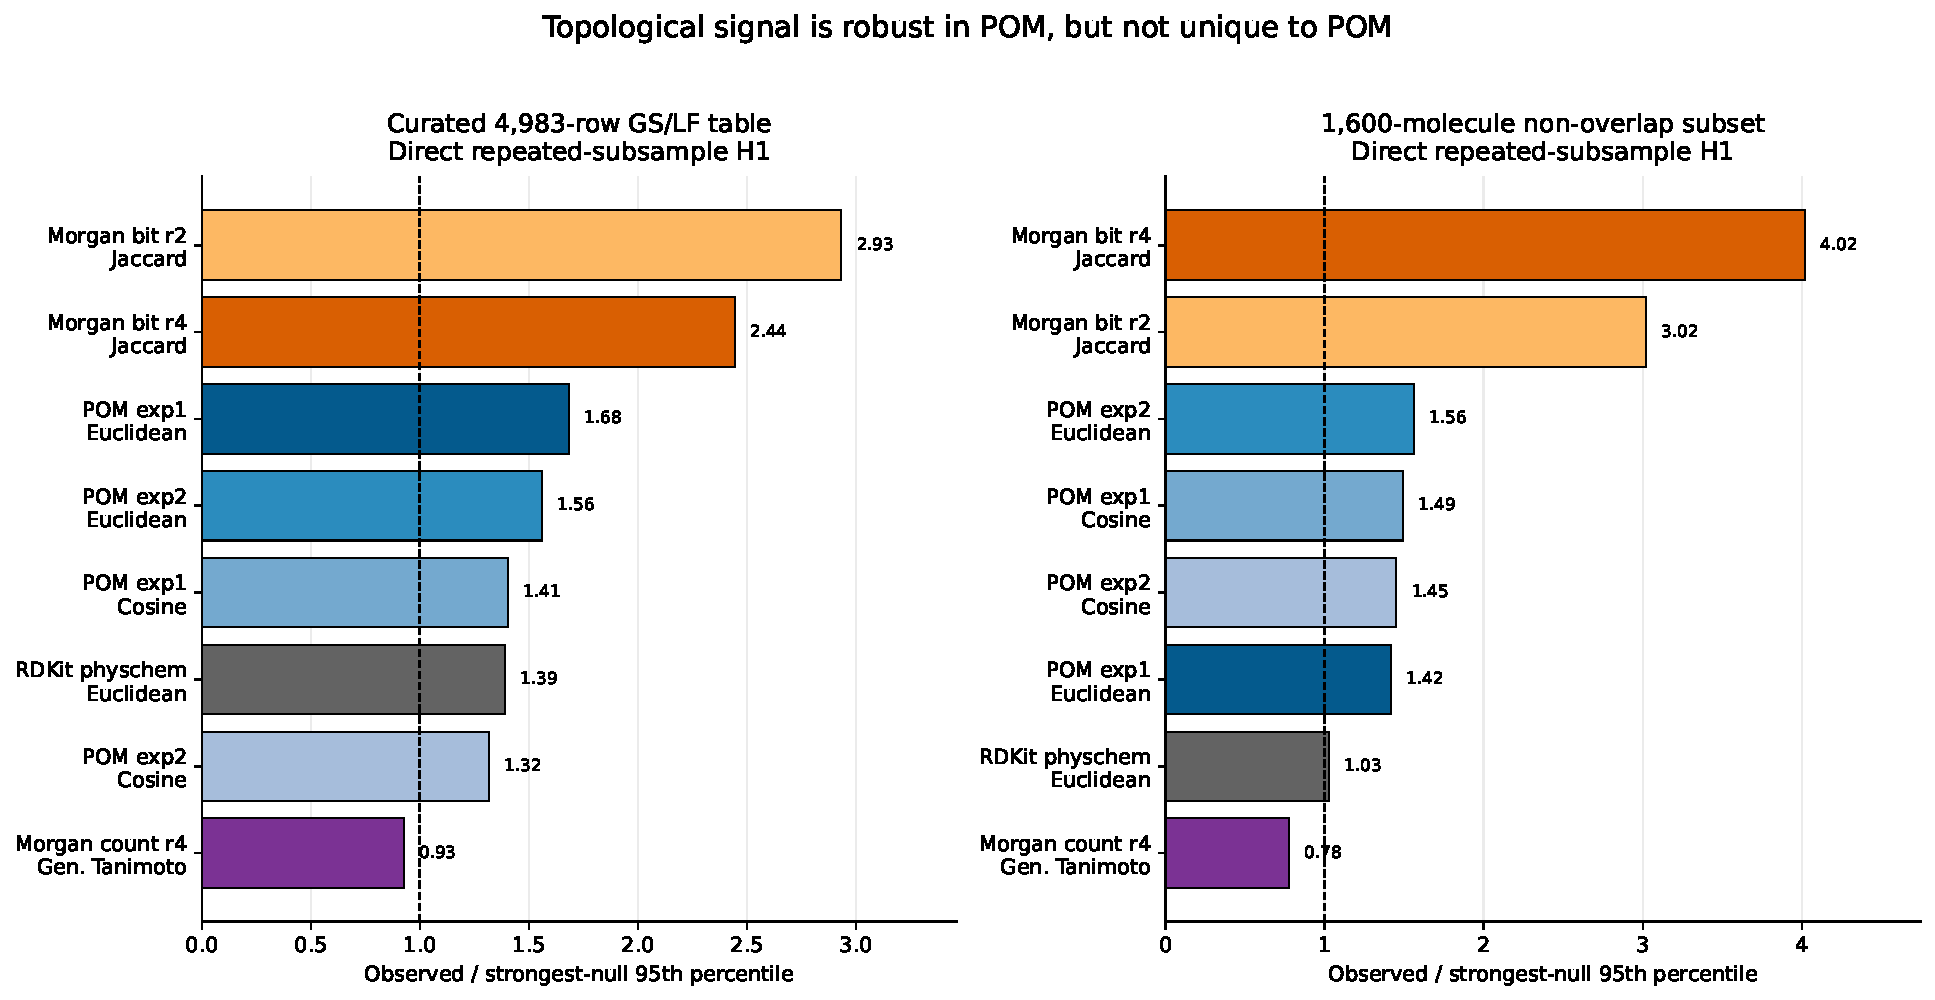
\includegraphics[width=\textwidth]{figures/figure1_direct_robustness.pdf}
  \caption{Direct repeated-subsample $H_1$ robustness on the curated table and the non-overlap subset. The dashed line marks the null threshold ratio of 1.0. POM is robust in both datasets, but the strongest direct signal belongs to Morgan bit fingerprints rather than POM.}
  \label{fig:direct}
\end{figure}

\subsection{Strong baselines prevent a uniqueness claim}

The strongest result in this study is not that POM contains no topological signal. The strongest result is that robust signal is not uniquely favorable to POM. On the curated table, paper-matched Morgan bit fingerprints (radius 4, 2048 bits) reached a direct top-1 ratio of 2.445, well above the primary POM values. On the non-overlap subset the same baseline reached 4.021, again exceeding both POM checkpoints.

The second-route landmark analysis preserved the same qualitative caution (Figure~\ref{fig:landmark}). On the curated dataset, landmarked Euclidean POM remained above null at 1.335, but landmarked cosine POM was borderline at 0.991 for the primary checkpoint and below threshold at 0.919 for the replication checkpoint. On the non-overlap subset, the landmarked POM cosine signal became healthier (1.091 and 1.132 for the two checkpoints), yet Morgan bit fingerprints remained stronger at 1.971.

This combination of results supports the statement ``topological signal in POM is real'' while rejecting the stronger statement ``POM uniquely captures odor-space topology better than strong chemical baselines.''

\begin{figure}[H]
  \centering
  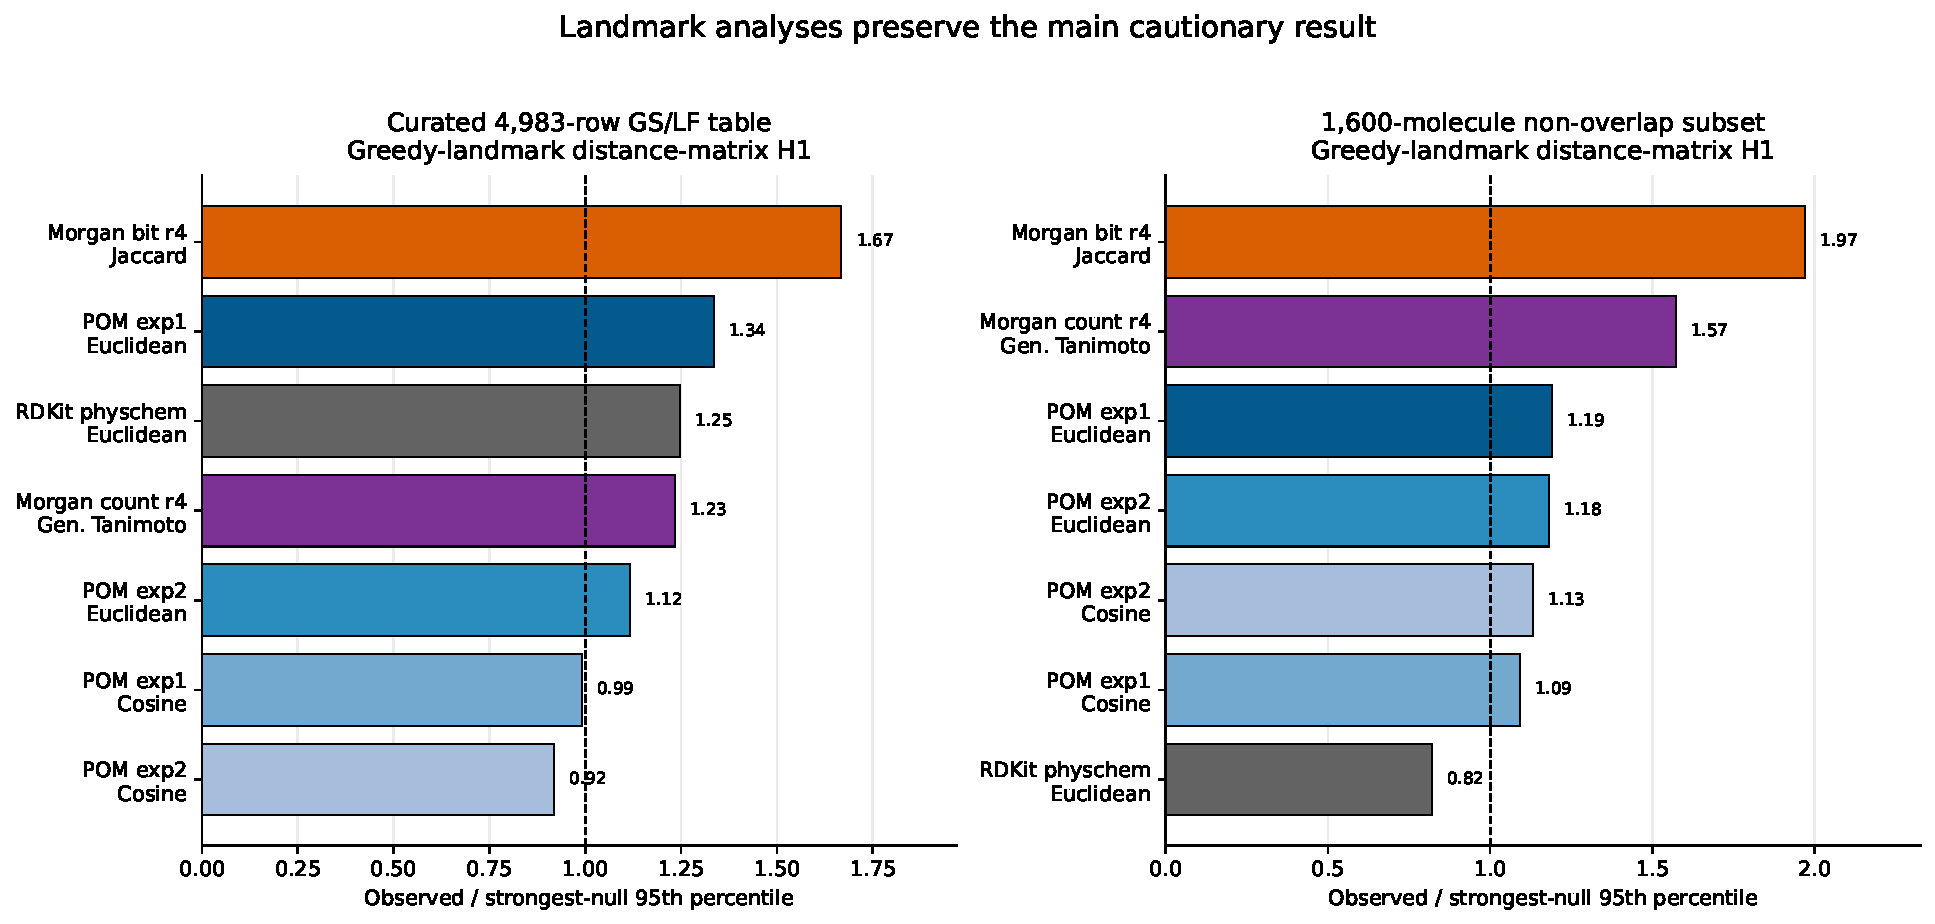
\includegraphics[width=\textwidth]{figures/figure2_landmark_robustness.pdf}
  \caption{Greedy-landmark distance-matrix analyses. The landmark route makes the curated cosine POM result more cautious while preserving the broader conclusion that robust signal is not unique to POM.}
  \label{fig:landmark}
\end{figure}

\subsection{Compression makes the POM result more interesting, but not more conclusive}

An important interpretive detail is that POM is also a substantially more compressed representation than the main fingerprint baselines used here. In these experiments, the learned POM embeddings are 256-dimensional dense vectors, whereas the matched Morgan fingerprint baselines are 2048-dimensional sparse encodings of explicit substructure content. That difference is not only numerical. It also reflects a difference in representational granularity: Morgan fingerprints preserve fine combinatorial chemical detail directly, while POM is a learned, lower-dimensional abstraction intended to organize odor-relevant information.

This matters because stronger topological signal in a fingerprint space does not automatically imply that the fingerprint contains more \emph{odor-relevant} structure. It may partly reflect the fact that sparse high-dimensional substructure encodings naturally preserve scaffold discreteness, substitution boundaries, and other combinatorial regularities that can produce persistent features under Jaccard- or Tanimoto-style geometries. By contrast, a learned dense representation may smooth or compress those regularities while still retaining enough structure to remain robust under repeated topological analyses.

For that reason, one scientifically careful way to read the present results is the following:

\begin{itemize}
  \item the Morgan baselines exhibit stronger topological signal relative to their own matched nulls;
  \item POM nevertheless retains reproducible nontrivial signal despite substantial dimensional and informational compression;
  \item this makes the POM result nontrivial, but it does not rescue a uniqueness claim;
  \item to show that the compressed representation preserves \emph{better} odor-relevant structure, one would need external evidence such as stronger alignment to receptor-response organization, stronger odor-label utility, or better downstream behavior in generation or search.
\end{itemize}

The present study only partially addresses that last point. The local utility analysis suggests that topology-derived features in POM can help for some odor-neighborhood targets, especially on the curated dataset, but the gains are modest and not uniquely favorable to POM. A stronger future version of this argument would compare POM to dimension-matched or bottleneck-matched chemical baselines, rather than only to much larger sparse representations.

\subsection{Checkpoint-to-checkpoint variation changes scale, not the main conclusion}

An obvious concern is that the observed signal could depend on one favorable checkpoint. Figure~\ref{fig:ensemble} addresses this concern by summarizing all 10 released OpenPOM ensemble checkpoints. Euclidean top-1 signal-to-null ratios remained above threshold for all checkpoints, with mean 1.522, minimum 1.424, and maximum 1.685. Cosine ratios were slightly weaker but still mostly stable, with mean 1.363, minimum 1.142, and maximum 1.545; 9 of 10 checkpoints achieved a minimum run fraction of 1.0 above null, while one reached 0.875.

Distance geometry also remained similar across checkpoints. Across 45 pairwise checkpoint comparisons, sampled pairwise-distance Pearson correlations had mean 0.808, minimum 0.753, and maximum 0.861. Taken together, these results support a stable Euclidean story and a somewhat more metric-sensitive cosine story.

\begin{figure}[H]
  \centering
  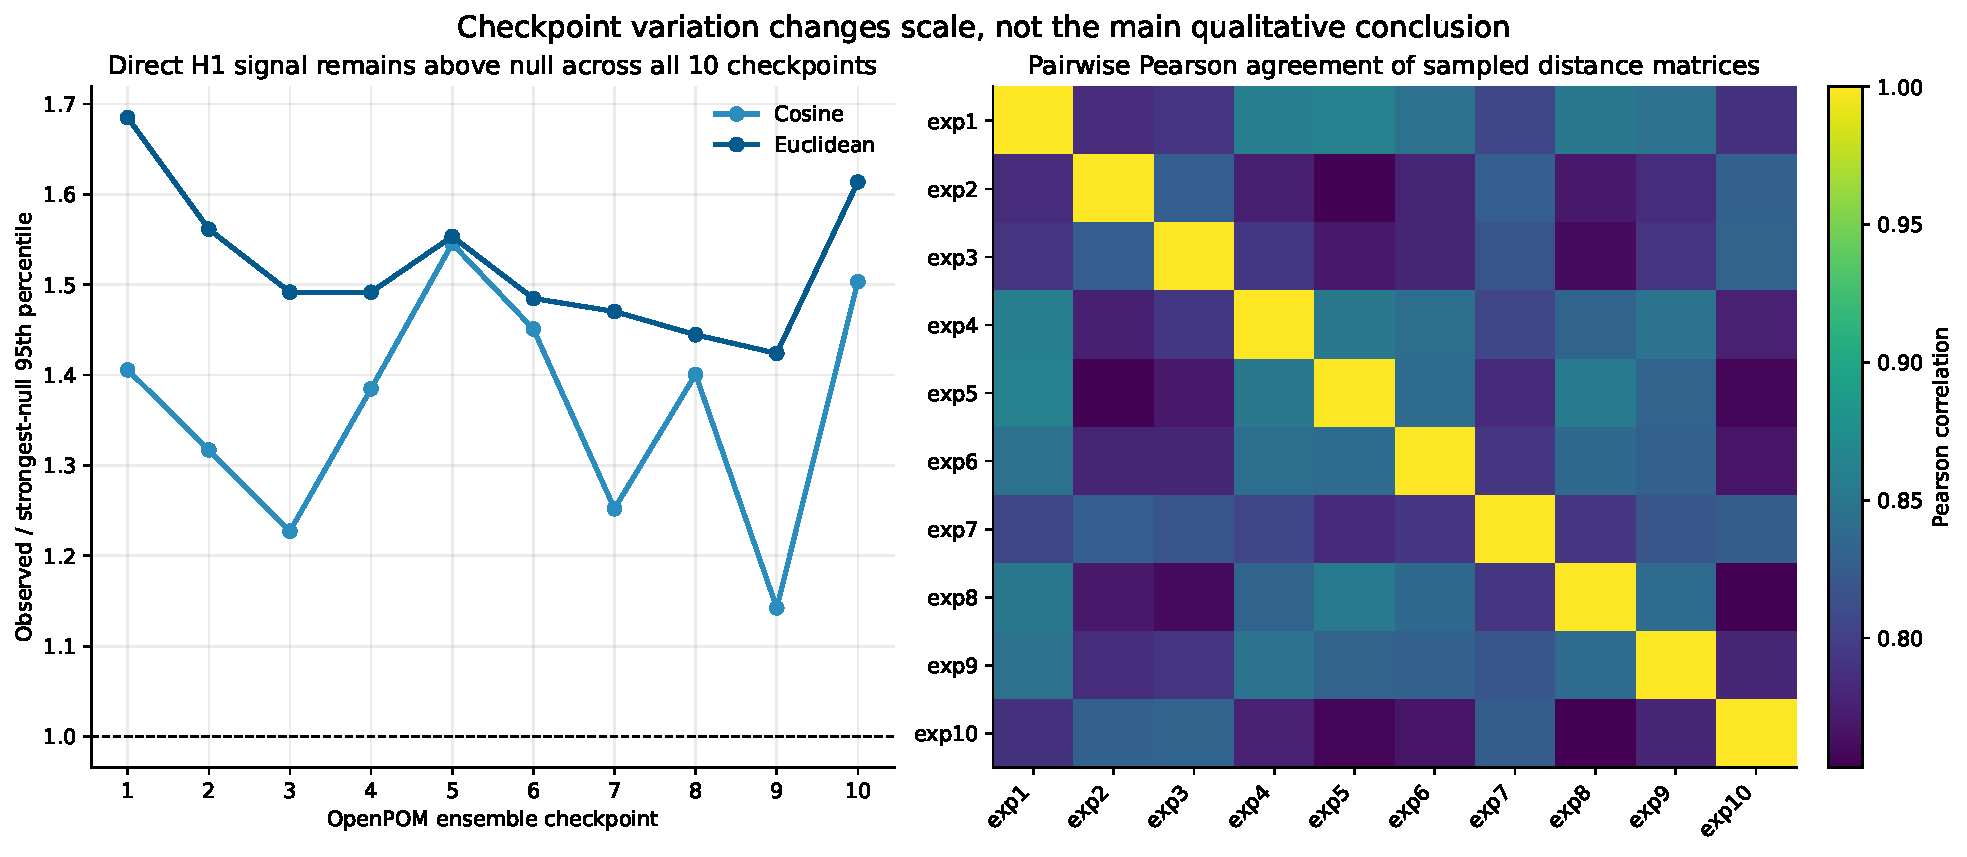
\includegraphics[width=\textwidth]{figures/figure3_ensemble_stability.pdf}
  \caption{Checkpoint stability across the full released OpenPOM ensemble. Left: direct top-1 signal-to-null ratios for cosine and Euclidean metrics. Right: pairwise Pearson agreement of sampled distance matrices across checkpoints.}
  \label{fig:ensemble}
\end{figure}

\subsection{Topology can add utility, but gains are modest and not POM-specific}

The utility analysis was designed to ask a narrower question than ``does topology matter for molecular design?'' Specifically, does local topology add explanatory value beyond local geometry for neighborhood-level odor-label summaries? The answer is cautiously yes, but only in a limited and target-dependent sense.

On the curated table, the strongest POM gains came from the cosine representation: adding topology increased mean $R^2$ by 0.0476 for neighbor-label entropy and by 0.0415 for share-any-label fraction. On the non-overlap subset, the largest POM gain was smaller, 0.0220 for neighbor-label entropy under cosine. At the same time, some of the best utility gains on the non-overlap subset came from non-POM representations, including RDKit physicochemical descriptors (0.0414 for neighbor-label entropy) and Morgan count fingerprints (0.0383 for share-any-label fraction).

Figure~\ref{fig:utility} therefore supports a restrained conclusion: topology-derived local features sometimes help, but the effect is not universal, not obviously large, and not uniquely associated with POM.

\begin{figure}[H]
  \centering
  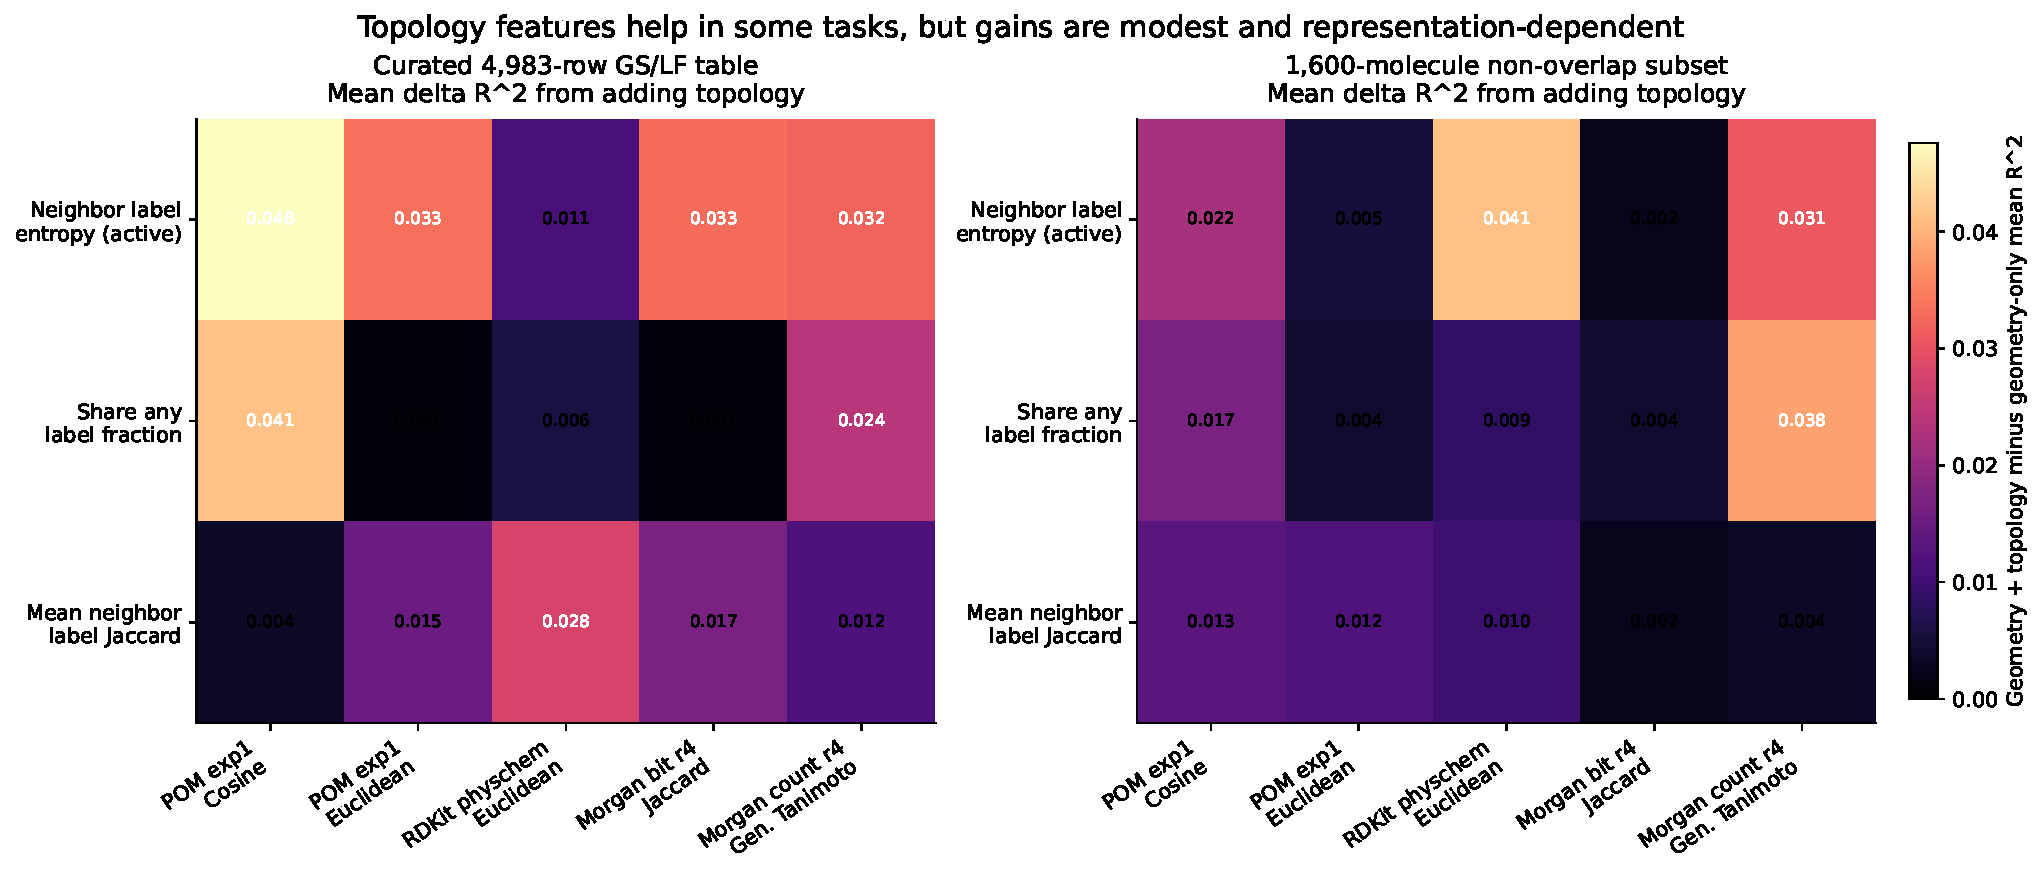
\includegraphics[width=\textwidth]{figures/figure4_utility_deltas.pdf}
  \caption{Mean $\Delta R^2$ from adding topology to geometry-only local models. Improvements are real in several settings, especially for entropy-related targets, but they are modest and representation-dependent rather than uniquely favorable to POM.}
  \label{fig:utility}
\end{figure}

\section{What This Analysis Supports}

The present results support the following claims:

\begin{itemize}
  \item POM embeddings exhibit reproducible $H_1$ signal under repeated direct analyses on multiple odor datasets.
  \item Euclidean POM signal is stable across released OpenPOM checkpoints.
  \item Landmark analyses broadly agree with the direct route, while also revealing that the cosine story is more metric-sensitive than the Euclidean story.
  \item Local topology features can improve neighborhood-level odor-label prediction beyond local geometry in some settings.
\end{itemize}

\section{What This Analysis Does Not Support}

The results do \emph{not} support stronger claims that would be easy to overstate:

\begin{itemize}
  \item They do not establish that current learned odor embeddings possess topology that is uniquely favorable relative to strong chemical baselines.
  \item They do not imply that detected loops correspond to interpretable cyclic perceptual dimensions.
  \item They do not show that topology-derived features confer broad practical utility for molecular design or other application-heavy tasks.
  \item They do not yet separate ``odor-relevant structure preserved under compression'' from ``raw combinatorial structure retained by sparse chemical encodings'' as cleanly as a dimension-matched baseline study would.
  \item They do not yet provide feature-level matching or persistence-image stability analyses beyond top-$k$ persistence summaries.
\end{itemize}

\section{Limitations and Immediate Next Steps}

This study is strongest as a representation audit. It remains limited by its narrow utility targets, its focus on $H_1$, and the use of a single utility model family (ridge regression). The most defensible next steps are therefore incremental rather than grand:

\begin{itemize}
  \item add a richer stability analysis beyond top-$k$ persistence magnitudes;
  \item add dimension-matched or bottleneck-matched chemical baselines for a cleaner compression-sensitive comparison;
  \item test whether the utility conclusions survive a second model family;
  \item consider a block-permutation test for topology feature sets;
  \item optionally extend the non-overlap subset checkpoint analysis from two checkpoints to all 10 released ensemble members.
\end{itemize}

\section{Reproducibility}

This manuscript is tied directly to repository artifacts rather than an ad hoc notebook narrative. The figures in this draft are generated from CSV and JSON reports in \texttt{outputs/reports/} via \texttt{scripts/14\_make\_arxiv\_figures.py}. The repository snapshot associated with this draft is available at \url{https://github.com/Obiohagwu/odor-topology}. The current arXiv source bundle is stored in \texttt{arxiv/}. Because the local machine used for packaging did not have a TeX toolchain installed, this draft was prepared as source without local PDF compilation.

\section{Conclusion}

The main conclusion is intentionally modest. Topological data analysis does reveal reproducible structure in learned odor embeddings, and that signal is stable enough to merit attention. At the same time, robust signal is not uniquely attributable to POM, and practical utility gains remain conditional. The value of this work is therefore not in claiming a new theory of odor space. Its value is in clarifying what the current evidence does and does not justify, while providing a reusable evaluation pipeline for future representation studies.

\begin{thebibliography}{9}

\bibitem{lee2023pom}
B. K. Lee, E. J. Mayhew, B. Sanchez-Lengeling, J. N. Wei, W. W. Qian, K. A. Little, M. Andres, B. B. Nguyen, T. Moloy, J. Yasonik, J. K. Parker, R. C. Gerkin, J. D. Mainland, and A. B. Wiltschko.
\newblock A principal odor map unifies diverse tasks in olfactory perception.
\newblock \emph{Science}, 381(6661):999--1006, 2023.
\newblock doi: \href{https://doi.org/10.1126/science.ade4401}{10.1126/science.ade4401}.

\bibitem{barsainyan2023openpom}
A. A. Barsainyan, R. Kumar, P. Saha, and M. Schmuker.
\newblock OpenPOM: open-source principal odor map models for olfaction.
\newblock Software repository, 2023.
\newblock \url{https://github.com/BioMachineLearning/openpom}. Accessed April 7, 2026.

\bibitem{edelsbrunner2008persistent}
H. Edelsbrunner and J. Harer.
\newblock Persistent homology---a survey.
\newblock In J. E. Goodman, J. Pach, and R. Pollack, editors, \emph{Surveys on Discrete and Computational Geometry: Twenty Years Later}, volume 453 of \emph{Contemporary Mathematics}, pages 257--282. American Mathematical Society, 2008.
\newblock doi: \href{https://doi.org/10.1090/conm/453/08802}{10.1090/conm/453/08802}.

\bibitem{ghrist2008barcodes}
R. Ghrist.
\newblock Barcodes: the persistent topology of data.
\newblock \emph{Bulletin of the American Mathematical Society}, 45(1):61--75, 2008.
\newblock doi: \href{https://doi.org/10.1090/S0273-0979-07-01191-3}{10.1090/S0273-0979-07-01191-3}.

\bibitem{morgan1965generation}
H. L. Morgan.
\newblock The generation of a unique machine description for chemical structures---a technique developed at Chemical Abstracts Service.
\newblock \emph{Journal of Chemical Documentation}, 5(2):107--113, 1965.
\newblock doi: \href{https://doi.org/10.1021/c160017a018}{10.1021/c160017a018}.

\bibitem{bauer2021ripser}
U. Bauer.
\newblock Ripser: efficient computation of Vietoris--Rips persistence barcodes.
\newblock \emph{Journal of Applied and Computational Topology}, 5:391--423, 2021.
\newblock doi: \href{https://doi.org/10.1007/s41468-021-00071-5}{10.1007/s41468-021-00071-5}.

\bibitem{landrum2006rdkit}
G. Landrum et al.
\newblock RDKit: Open-source cheminformatics software.
\newblock \url{https://www.rdkit.org}, 2006--.
\newblock Accessed April 7, 2026.

\end{thebibliography}

\end{document}
